% ****** Start of file apssamp.tex ******
%
%   This file is part of the APS files in the REVTeX 4.1 distribution.
%   Version 4.1r of REVTeX, August 2010
%
%   Copyright (c) 2009, 2010 The American Physical Society.
%
%   See the REVTeX 4 README file for restrictions and more information.
%
% TeX'ing this file requires that you have AMS-LaTeX 2.0 installed
% as well as the rest of the prerequisites for REVTeX 4.1
%
% See the REVTeX 4 README file
% It also requires running BibTeX. The commands are as follows:
%
%  1)  latex apssamp.tex
%  2)  bibtex apssamp
%  3)  latex apssamp.tex
%  4)  latex apssamp.tex
%

\documentclass[%
 reprint,
%superscriptaddress,
%groupedaddress,
%unsortedaddress,
%runinaddress,
%frontmatterverbose, 
%preprint,
%showpacs,preprintnumbers,
%nofootinbib,
%nobibnotes,
%bibnotes,
 amsmath,amssymb,
%  aps,
pra,
%prb,
%rmp,
%prstab,
%prstper,
%floatfix,
]{revtex4-1}

\usepackage{graphicx}% Include figure files
\usepackage{dcolumn}% Align table columns on decimal point
\usepackage{bm}% bold math
\usepackage{mathrsfs}
\usepackage{amsmath}
\usepackage{bbm}
\usepackage{wrapfig}
\usepackage{bm} 
\usepackage{amssymb}
\usepackage{tikz}
%\usepackage{hyperref}% add hypertext capabilities
%\usepackage[mathlines]{lineno}% Enable numbering of text and display math
%\linenumbers\relax % Commence numbering lines

%\usepackage[showframe,%Uncomment any one of the following lines to test 
%%scale=0.7, marginratio={1:1, 2:3}, ignoreall,% default settings
%%text={7in,10in},centering,
%%margin=1.5in,
%%total={6.5in,8.75in}, top=1.2in, left=0.9in, includefoot,
%%height=10in,a5paper,hmargin={3cm,0.8in},
%]{geometry}
\usepackage{listings}
\usepackage{color}
\usepackage{subfigure}

\begin{document}

\preprint{APS/123-QED}

\title{A quantum algorithm for solving computational fluid dynamics problems}

\author{Zhao-Yun Chen}
%  \altaffiliation[Also at ]{Physics Department, XYZ University.}%Lines break automatically or can be forced with \\
 \affiliation{Key Laboratory of Quantum Information, CAS}
 \affiliation{Origin Quantum Computing, Hefei, China}
 \email{agony@mail.ustc.edu.cn}
\author{Cheng Xue}%
 \affiliation{Key Laboratory of Quantum Information, CAS}
 \email{itachi@mail.ustc.edu.cn}
\author{Si-Ming Chen}
 \affiliation{Key Laboratory of Quantum Information, CAS}
\author{Bin-Han Lu}
 \affiliation{Key Laboratory of Quantum Information, CAS}
\author{Ye Li}
 \affiliation{Origin Quantum Computing, Hefei, China}
\author{Ning-Bo An}
 \affiliation{Origin Quantum Computing, Hefei, China}
\author{Zhi-Xing Zhu}
 \affiliation{Origin Quantum Computing, Hefei, China}
\author{Sheng-Hong Huang}
\affiliation{School of Engineering Science, USTC}
\author{Ju-Chun Ding}
\affiliation{Department of Modern Mechanics, USTC}

\author{Guo-Ping Guo}
\affiliation{Key Laboratory of Quantum Information, CAS}
\email{gpguo@mail.ustc.edu.cn}
% \affiliation{%
%  Authors' institution and/or address\\
%  This line break forced with \textbackslash\textbackslash
% }%

% \collaboration{MUSO Collaboration}%\noaffiliation

% \author{Charlie Author}
%  \homepage{http://www.Second.institution.edu/~Charlie.Author}
% \affiliation{
%  Second institution and/or address\\
%  This line break forced% with \\
% }%
% \affiliation{
%  Third institution, the second for Charlie Author
% }%
% \author{Delta Author}
% \affiliation{%
%  Authors' institution and/or address\\
%  This line break forced with \textbackslash\textbackslash
% }%

% \collaboration{CLEO Collaboration}%\noaffiliation

\date{\today}% It is always \today, today,
             %  but any date may be explicitly specified

\begin{abstract}
    Computational fluid dynamics (CFD) is a branch of fluid mechanics that uses numerical computation to analyze fluid flows. When the number of mesh grows, the requirement of the computing resources becomes more expensive. Here, we propose a quantum algorithm to solve CFD problems, which exponentially faster than the classical solver. We analyzed the time complexity and requirement of qubit resources of our algorithm and simulated a specific CFD problem to prove the result.

\end{abstract}

\pacs{Valid PACS appear here}

\maketitle

\section{Introduction}
Quantum computing is promising to have wide application on various computational tasks. It is believed that quantum computing has potentially exponential acceleration over the classical approach. There have already been many quantum algorithms to prove this idea: quantum factorization, quantum simulation, linear problem solver, etc. 

Quantum computing has “quantum parallism”. An n-qubit quantum state is a vector in $C^{2^n}$ Hilbert space (a complex linear space). Every quantum operation is a transformation in the such linear space. If the quantum state vector encodes the description to a realistic problem, we can handle the whole vector with one operation in parallel without iterating over them. For example, if we want to multiply a matrix and vector, we no longer need for-loops, but with a few quantum gates directly applying on the input quantum states. This feature enables a group of algorithms called quantum linear algebra, which are exponentially faster than the classical algorithm.

Computational Fluid Dynamics (CFD) problems are often related to solving a series of equations in numerical methods. Here we do not introduce the classical CFD method. But we need to mention that a CFD solver needs to do time integration on the partial derivative equations, so that it needs to iterate with a $\Delta t$ to calculate a small evolution of the system, and finally stops when the system goes stable. In this problem set, we should understand the SU2 solver and try to replace some modules with quantum subroutines, (a.k.a. quantum-classical hybrid approach,) to seek quantum speed-up in this problem.

Here we introduce our algorithm. The modules that we replace are data structures used and methods called in the class CFluidIteration. In the data structure, these are replaced by quantum memory or quantum states: including the information about the mesh grid and all vectors that are involved in the linear equations. In the process of the time integration, the linear solver is replaced by a quantum version. And in other pro- and post-processing parts, they are completely replaced by quantum arithmetic modules to form the oracle necessary in the quantum linear solver. Besides, we do not change the problem model, the mesh setting and the FVM method, including the iteration process of the time integration. 

As the result, the time complexity of our algorithm is proportional to $\log⁡ N$, where N denotes the mesh number. The qubit number is also proportional to $\log⁡ N$. Besides the effect of the mesh number, both the complexity and the qubit number are affected by the precision $\epsilon$. We also dicussed the conditional number and the sparsity. They affect the time complexity, however, they are considered as a constant in the problem because they will not change greatly.

Along with the algorithm detail, we also discuss the difficulties of the problem. One is that we prove that it is necessary to include the quantum random access memory (QRAM), without which quantum speed up will not be achieved. Another is that the qubit should be fault-tolerant logical qubit, because the requirements of the gate number and the state storage time greatly exceed any limit of the near-future NISQ device.

\section{Submission Summary}

\subsection{Replacement of the SU2 submodule}

SU2 is an open-source fluid dynamics solver. We study its SU2\_CFD module to solve the computational fluid dynamic problem and the target is to replace some modules in the classical solver by quantum subprocess to form a quantum-classical hybrid software, finally to demonstrate the quantum speed-up. Here is the modules we replace in the SU2 solver.

Process: MultiGrid\_Cycle and Preprocessing in the CFluidIteration.

Data Structure: class CGeometry and CNumerics

\begin{figure*}[htbp]
    \subfigure{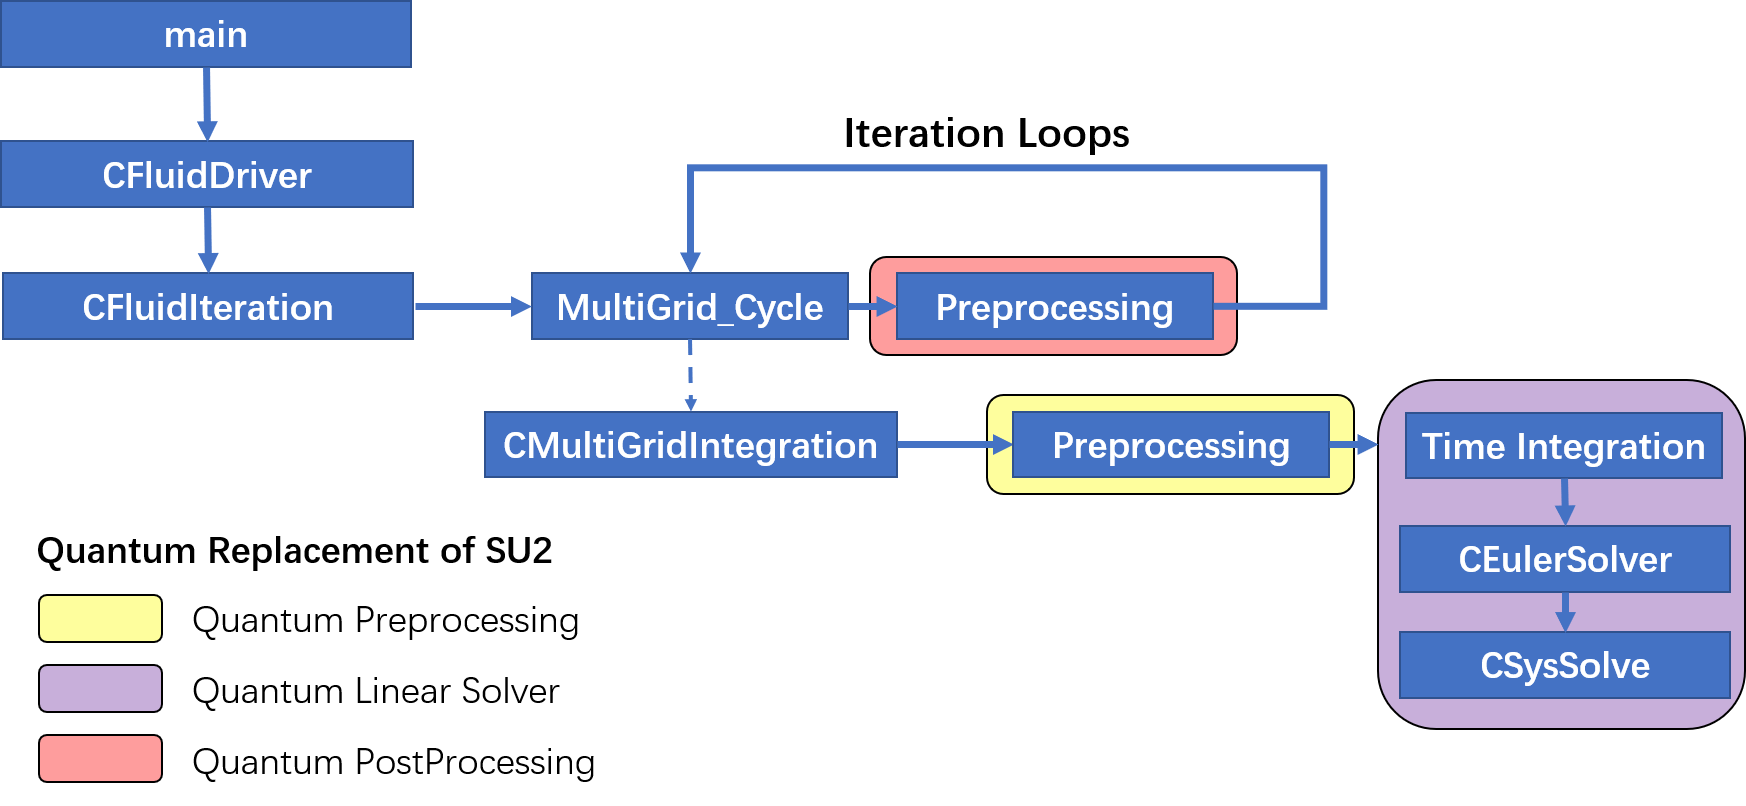
\includegraphics[width=0.95\textwidth]{Fig/SU2_process.png}}
     \caption{SU2 modules.}
    \label{SU2modules}
\end{figure*}

The preprocessing in the CMultiGridIntegration includes the preprocess about the generation of the linear problem. This part is replaced by quantum arithmetic and calling to the oracle holding the data of the mesh information. The final target, similar to the classical process, is to generate the quantum data needed in the next step: Quantum linear solver.

MultiGrid\_Cycle calls the TimeIntegration method in the CMultiGridIntegration, which is replaced by quantum linear solver. The quantum linear solver is exponentially faster than the classical counterpart. The SpaceIntegration is no longer needed because it is automatically handled by the quantum parallism.

The preprocessing in the CFluidIteration handles the result after the MultiGrid\_Cycle, generates the data for the next iteration, and displays the result. This module is replaced by a quantum postprocess, which aims to add the variation to the vector and to prepare the next iteration. 

\subsection{Overview of the algorithm}

\begin{figure}[htbp]
	\subfigure{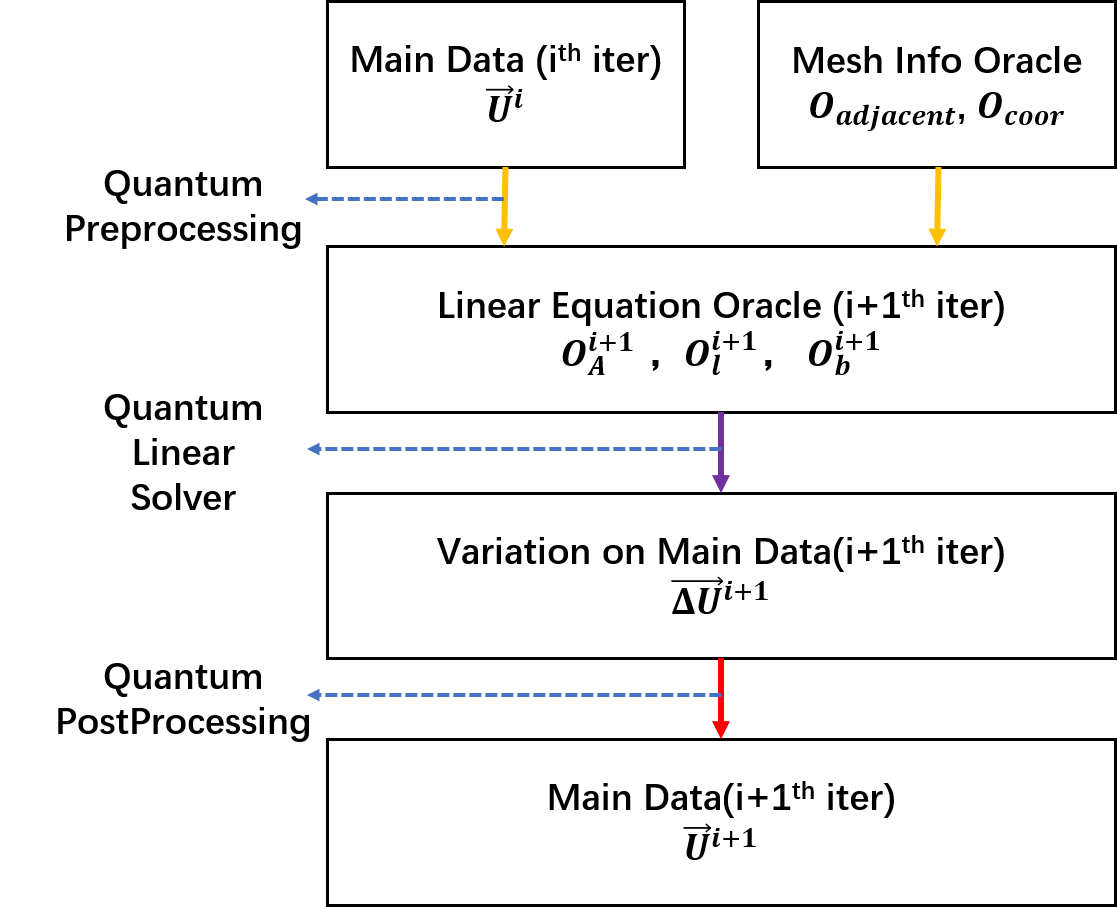
\includegraphics[width=0.45\textwidth]{Fig/QuantumProcess.png}}
    \caption{Processes in an iteration step}
    \label{QuantumProcess1} 
\end{figure}

As in Fig. 1, we marked the modules that we replace in our algorithm. With corresponding to the Fig. 2, the yellow part is replaced by the Quantum Preprocessing, the violet by the Quantum Linear Solver and the red by the Quantum PostProcessing. The quantum processes in each iteration step are doing a step of the time integration of $\Delta t$, with inputting $\vec{u}^i$ and outputting $\vec{u}^{i+1}$. We here have
$$
u^0=u^0(initializer)
$$
$$
A=A(\vec{U}^{i-1},\hat{M})
$$
$$
x=\Delta \vec{U}^i
$$
$$
b=b(\vec{U}^{i-1},\hat{M})
$$
$$
\vec{U}^i=\vec{U}^{i-1}+\Delta \vec{U}^i
$$
where $M$ denotes the given information of the mesh grid. In each iteration step, the coefficient matrix and the constant vector of the linear equation are related to the solution of the previous step. 

\subsection{Comparing quantum approach with classical approach}

\subsubsection{Classical Solver}

The implicit Euler solver has the linear complexity. We declare this result with two proofs: in both theory and experiment. The theory shows that the classical solver uses multigrid method, which are expected to have the complexity $O(n)$ where $n$ denotes the number of mesh grids. We also did experiment on various grid size and calculates the running time (except the preparation). As the figure shows, that running time has a very good linearity to the mesh number.
\begin{figure} 
\centering
\includegraphics[width=0.45\textwidth]{Fig/su2_speed.png}
\caption{SU2 running time.} \label{su2Speed}
\end{figure}

It is unclear whether the time integration can be cancelled to avoid the iteration process. We here do not change the iteration process, that is, we have to seek a quantum approach with sublinear runtime between each iteration step.

\subsubsection{Quantum Linear Solver}

We here use the quantum linear solver as the accelerator of the calculation. The first quantum linear solver was developed by Harrow, Hassidim and Lloyd. The algorithm solves the linear equation $Ax = b$, which requires $O((d log⁡N)/\epsilon)$ oracle query and has the successful rate with $O(1/\kappa)$ where N represents the dimension of the equation, $d$ the sparsity of the matrix, $\epsilon$ the target precision, and $\kappa$ the conditional number of the matrix A. The quantum solver is then improved by Andrew Childs’s works. In these works, the complexity dependencies on the precision, conditional number are changed from linear to logarithm. The works introduces a method of linear combination of the operators, which are inspired by the previous works about the duality quantum computing framework established by Long.

The solver requires an efficient quantum representation of the matrix A and constant b. In this problem, the set of the partial derivative equations should be linearized to generate the expression of A and b.

\subsubsection{Overall Complexity}

QRAM is necessary in model to demonstrate quantum speed up. We use QRAM in three procedures. First is to store the information about the mesh grid. Second is to store the interval results of the solver. Third is to help recover from the probabilistic error of performing a non-unitary transformation. Here we list the qubit,query and gate complexity of the whole process of our algorithm: the required qubit number is
$$
O(qnum)=O(2log(4N)+log(d\kappa log(d\kappa/\epsilon)))
$$
The QRAM and oracle query complexity is 
$$O(query)=O(d\kappa^2log^2(d\kappa/\epsilon))$$
The gate complexity is 
$$
O(d\kappa^2log^2(d\kappa/\epsilon)\times poly(log(4N)/\epsilon))
$$
In Sec.~\ref{detail}, we will analyze in detail the complexity of each module of our algorithm.

\begin{table*}
	\caption{Comparison of quantum approach and classical approach}\label{tab2}
	\resizebox{\textwidth}{!}{ \begin{tabular}{|c|c|c|c|c|}
	\hline 
	Iteration&Equation Solver&Data Between Each Step&Slowest Sub-procedure&Time complexity \\
	 & & & &(n denotes the number of mesh grid)\\
	\hline  
	Yes&Classical&Classical&Multigrid Linear Equation Solver&$O(n)$\\
	\hline 
	Yes&Quantum&Classical&Quantum Classical Converter&$O(n)$\\
	\hline 
	Yes&Quantum&Quantum&Quantum Linear System Solver (With QRAM)&$O(log(n))$\\
	\hline 
	Yes&Quantum&Quantum&Impossible to implement (Without QRAM)&$-$\\
	\hline 
	\end{tabular} }
\end{table*}

\subsection{Improvement for mesh generation}
Besides the acceleration in the time integration process, the mesh generation module can also be integrated in the quantum computer.

In the above algorithm, we considered the mesh information as the oracle. A direct way is to generate the mesh file beforehand, and encode the classical data into the quantum computer. This way may cause a time complexity of $O(N)$. Instead of reading a pre-generated mesh file, we could replace the mesh generation program by a quantum algorithm. This method will be discussed in the detailed explanation.

\subsection{Assumptions on the Future Quantum Computer}

To realize our quantum approach and the effect of the acceleration, we claim that several assumptions must be made on the future quantum computer.

\subparagraph{Fault-Tolerance}
Our algorithm accelerates the calculation in each iteration step, however, the number of iteration, as we investigated, would be much bigger when the number of the mesh grows. We do not perform quantum measurements to extract the result in each step. Instead, the quantum feature (entanglement, superposition) should be preserved during the whole calculation process. 

This feature of the algorithm implies the storage of the quantum state is not affected by the decoherence and noise. Only a fault-tolerant quantum computer can meet this demand.

\subparagraph{Quantum Random Access Memory}
The quantum-classical hybrid algorithms are always facing the problem of the data conversion between the classical and the quantum.

The problem is what the time complexity is to perform such conversions:
$$ \sum|addr\rangle|data\rangle\ (Quantum\ Memory) $$
and (classical memory written in C++ form)
$$ \text{vector<complex<double> > data}\ (Classical\ Memory) $$

A trivial way of the quantum-to-classical is to do with repeatedly measurements, or as people always mention "quantum tomography". The trivial classical-to-quantum is to encode the state preparation phase in the quantum circuit by using a group of controlled rotation operations. These ways are trivial because they consume $O(2^n)$ time, while we think it is not efficient. If the quantum-classical conversion is not implemented efficiently, many quantum algorithms will never realize the sublinear time complexity, because the input and the output will at least consume linear time.

To solve this problem, we have to assume the existence of the quantum random access memory (QRAM). The QRAM is a structure where we could save and load quantum information efficiently. Different as the trivial way, the QRAM operates the address in the superposition. It enables the digital form quantum data (compared to the analog form, as described in Supplementary Chapter QDAC/QADC) to be loaded and stored in parallel with the time complexity $O(log N)$.

Although the concept of the QRAM is proposed early and many works were based on this model, it is controversial whether a QRAM could exist, because the architecture of the QRAM remains an open question. We take this risk because we believe that if quantum computer wants to solve a realistic problem with sublinear complexity, the QRAM must exists. We will prove that this problem would not be sublinear without QRAM.

% \subsubsection{Advantages of the Algorithm}

% Advantages

% \subsubsection{Drawbacks of the Algorithm}



\section{Detailed Explanation}\label{detail}
In this section, we use the following symbols:

$N$: grid number

$m=log(4N)$

$q_f$:qubit number to represent a float number.

$IterTimes$: Iteration times

$|\vec{U}\rangle$: represents $\vec{U}=(\rho,\rho u, \rho\nu, \rho E)$, the dimension is $4N$. 

$\vec{u}_i$: variables of grid $i$ 

\subsection{FVM method}\label{classicalFVM}

An important applicaiton of modern Computational Fluid Dynamics (CFD) is to simulate systems in aircraft aerodynamic design. The usual classical algorithm often means high complexity, which forces us in seeking for more effective computations, e.g., a quantum-hybrid solution.

For briefness, we assumed the flow to be 2D, inviscid and steady, then gained Euler equations, a special form of the Navier-Stokes equation:
\begin{equation}
\left\{
\begin{array}{ccc}
	\frac{\partial \rho u}{\partial x} + \frac{\partial \rho v}{\partial y} & = & 0\\
	\rho u \frac{\partial u}{\partial x} + \rho v \frac{\partial u}{\partial y} & = & -\frac{\partial p}{\partial x}\\
	\rho u \frac{\partial v}{\partial x} + \rho v \frac{\partial v}{\partial y} & = & -\frac{\partial p}{\partial y}\\
	\rho u \frac{\partial H}{\partial x} + \rho v \frac{\partial H}{\partial y} & = & 0
\end{array}
\right.
\end{equation}

In these equations, we have the density $\rho$, the momentum $\rho\bm{V}=\left(\rho u, \rho v\right)$ and the enthalpy $H$, which were defined below:
\begin{equation}
\left\{
\begin{array}{ccc}
	H & = & c_p T + \frac{1}{2}\left(u^2 + v^2\right)\\
	p & = & \rho R T
\end{array}
\right.
\end{equation}
where $c_p = 1005 m^2 s^{-2} K^{-1}$ and $R = 287 m^2 s^{-2} K^{-1}$ are thermodynamical constants. The solution can also be considered as the stable situation of these equations \cite{hirsch2007numerical}:
\begin{align}\label{eq:differential_equation}
	\frac{\partial U}{\partial t} + \nabla \cdot \bm{F} = 0
\end{align}
\begin{equation}
\begin{array}{ccc}
U = \left[
\begin{array}{c}
\rho\\
\rho u\\
\rho v\\
\rho E
\end{array}
\right]
&
\bm{F}_x = \left[
\begin{array}{c}
\rho u\\
\rho u^2 + p\\
\rho u v\\
\rho u H
\end{array}
\right]
&
\bm{F}_y = \left[
\begin{array}{c}
\rho v\\
\rho u v\\
\rho v^2 + p\\
\rho v H
\end{array}
\right]
\end{array}
\end{equation}
\begin{align}
	E = \left(c_p - R\right) T + \frac{1}{2}\left(u^2 + v^2\right) = \frac{R T}{\gamma - 1} + \frac{1}{2}\left(u^2 + v^2\right)
\end{align}

For any volume $\Omega$ and its boundary $\partial\Omega$, Formula.\ref{eq:differential_equation} shows:
\begin{align}\label{eq:integral_equation}
	\frac{\partial}{\partial t}\int_\Omega U d V + \oint_{\partial \Omega} \bm{F} \cdot d \bm{S} = 0
\end{align}

One effective approach to solve the equation shown above is the Finite Volume Method (FVM). To solve the partial differential equations(PDE), discretization with numerical grid is necessary. Each spatial point is a node, identified by a set of indices, e.g. $\left(i, j\right)$ in the 2-D case, and several nodes combine a lattice. Midpoints of edges and centerpoints of adjacent lattices define a cell \cite{economon2015su2}. The equation of conservation was applied to each cell of the grid. With discretization of space, the calculus operations in PDE could also be changed to their numerical approximations. We chose implicit Euler scheme to deal with the time differential.
\begin{figure}[h]
	\centering  
	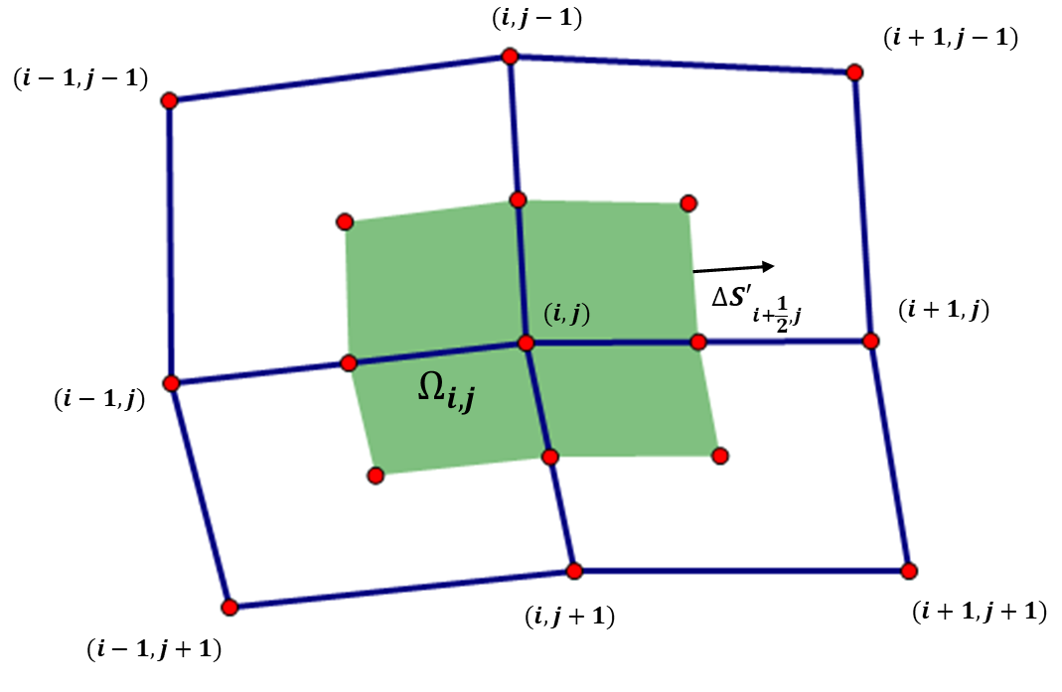
\includegraphics[width=0.7\linewidth]{Fig/grid}
	\caption{Sample of a octagonal cell with related nodes and quadrilateral lattices.}
	\label{fig:sample_of_cell}
\end{figure}

As illustrated in Figure.\ref{fig:sample_of_cell}, Formula.\ref{eq:integral_equation} was discretized to:
\begin{align}
	\frac{\Omega_{i, j}}{\Delta t}\left(U^{n+1}_{i, j}-U^{n}_{i, j} \right) = -\sum_{faces}\bm{F}^{n+1}\cdot\Delta\bm{S}^{n+1} = -R^{n+1}_{i, j}
\end{align}

Introduced to the concept of artificial dissipation, $\bm{F}^\prime_{i+\frac{1}{2}, j}$ matching with $\Delta\bm{S}^\prime_{i+\frac{1}{2}, j}$ satisfied \cite{hirsch2007numerical} \cite{jameson1981numerical}:
\begin{align}
\begin{split}
    \bm{F}^\prime_{i+\frac{1}{2}, j} =& \frac{1}{2}\left(\bm{F}_{i, j} + \bm{F}_{i + 1, j}\right) - \frac{1}{2}\big[\kappa^{\left(2\right)}\left(U_{i+1, j}-U_{i, j}\right)\\
    &+\kappa^{\left(4\right)}\left(U_{i+2, j}-3 U_{i+1, j}+3 U_{i, j}-U_{i-1, j}\right)\big]\\
    &\times\left[\frac{1}{2}\left(\bm{V}_{i, j} + \bm{V}_{i + 1, j}\right) + \sqrt{\gamma \frac{p}{\rho}}\frac{\Delta\bm{S}^\prime_{i+\frac{1}{2}, j}}{\left|\Delta\bm{S}^\prime_{i+\frac{1}{2}, j}\right|}\right]
\end{split}
\end{align}
where $\kappa^{\left(2\right)}$ and $\kappa^{\left(4\right)}$ are arbitrary non-dimensional coefficients, which we assumed to be $\frac{1}{2}$ and $\frac{1}{64}$.\\
Let $\Delta U^{n}$ be equal to $U^{n+1}-U^{n}$, and consider the $k-th$ components of $U$ \cite{economon2015su2}:
\begin{align}
	\left(\frac{\Omega_{i, j}}{\Delta t}\delta_{i, i^\prime}\delta_{j, j^\prime}+\left.\frac{\partial R_{i,j,k}}{\partial U_{i^\prime,j^\prime,k^\prime}}\right|_{U=U^n}\right)\Delta U^{n}_{i^\prime,j^\prime,k^\prime} = -R^{n}_{i,j,k}
\end{align}

We got an iterative problem with solving linear systems ($\mathcal{A} \Delta U = \bm{b}$). The residual $R^{n}$ tended toward zero, then the stable solution ($\frac{\partial U}{\partial t} = 0$) would be gained. And the quantum algorithms are effective at solving linear systems. We could build quantum circuits to accomplish the calculation. As against indulging in classical methods, fetching the quantum superiority might be more attractive.



\subsection{Initialization}

The Initialization process contains 2 steps: state initialization and meshing scheme oracle initialization.
\subsubsection{State initialization}
The initial value of  each $\vec{u}_i$ is the same, we assume the initial value of $\vec{u}_i$ in each grid can be written as $\vec{u}_i=(x_0,x_1,x_2,x_3)$, so the initial state  $|\vec{U}^0\rangle$ can be written as:
$$
|\vec{U}^0\rangle=C_0\sum_{i=0}^{4N-1}{x_{i\%4}|i\rangle}
$$
where $C_0=\frac{1}{\sqrt{N\sum_{i=0}^{3}{x_i^2}}}$, $|\vec{U}^0\rangle$ can be prepared with a $O(1)$ length quantum circuit, the quantum circuit is shown in fig.~\ref{state_initialization}.

\begin{figure}[htbp]
    \subfigure{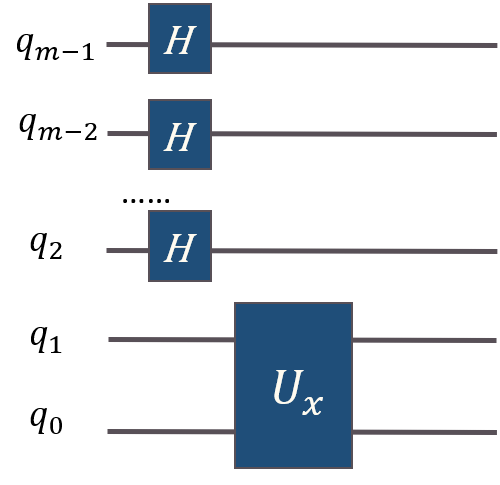
\includegraphics[width=0.30\textwidth]{Fig/state_initialization.png}}
    \caption{State initialization process.  }
    \label{state_initialization}
\end{figure}
Similarly, we can also construct the digital version of $\vec{U}^0$, which is written as:
$$
|\vec{d}_U^0\rangle=\sum_i{|i\rangle|U_i\rangle}
$$
the corresponding quantum circuit of $|\vec{d}_U^0\rangle$ is shown in fig.~\ref{digit_state_initialization}.In this process, we need $2m$ qubits and gete complexity is $O(1)$.

\begin{figure}[htbp]
    \subfigure{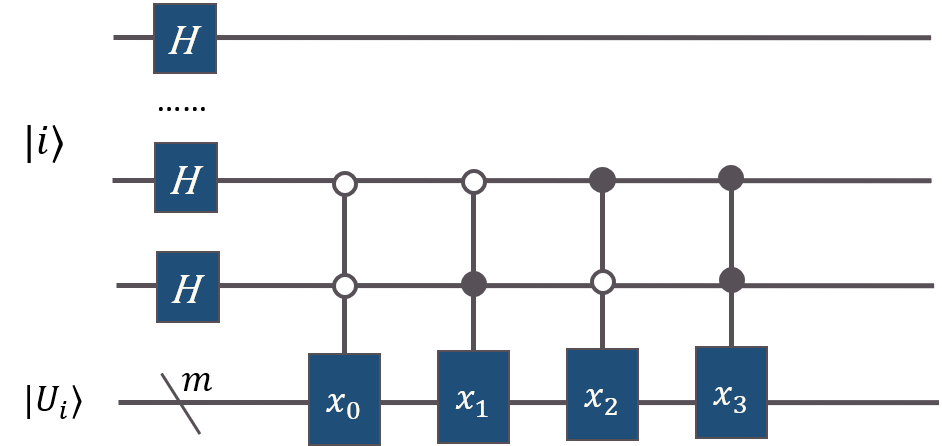
\includegraphics[width=0.30\textwidth]{Fig/digit_state.png}}
    \caption{Digital version of $\vec{U}^0$. }
    \label{digit_state_initialization}
\end{figure}

In the following process, we need a QRAM to store $|\vec{d}_U^0\rangle$, which is defined as:
$$
M_U|i\rangle|0\rangle=|i\rangle|U_i\rangle
$$
And $M_U$ can operate on a superposition state:
$$
M_U\frac{1}{\sqrt{4N}}\sum_i{|i\rangle|0\rangle}=\frac{1}{\sqrt{4N}}\sum_i{|i\rangle|U_i\rangle}
$$

\subsubsection{Meshing scheme oracle}

Meshing scheme oracle is used to encode meshing scheme into quantum circuit. We define two meshing scheme oracles: $O_{adjacent}$ and $O_{coor}$. $O_{adjacent}$ is used to extract the adjacent grid number of a specific grid, it can be writen as:
$$
O_{adjacent}|i\rangle|j\rangle=|i\rangle|g(i,j)\rangle
$$
it means $j-th$ adjacent grid number of grid $i$ is $g(i,j)$. $O_{coor}$ is used to extract coordinates of a grid:
$$
O_{coor}|i\rangle|0\rangle=|i\rangle|\vec{x}_i\rangle
$$
Here $\vec{x}_i$ means the coordinates of each corner of the grid $i$. We can get other position information with $O_{coor}$, such as grid center of gravity coordinates, the normal to each side of the grid $i$ and so on.

The number of qubits required to construct $O_{adjacent}$ and $O_{coor}$ is $2(m-2)$, $m-2+C_0q_f$ respectively, here $C_0q_f$ is a qubit sequence represents coordinate information and other position information obtained from grid coordinates, and $C_0$ is a constant number.

The construction complexity of $O_{adjacent}$ and $O_{coor}$ is related to the complexity of the meshing scheme. In our method, we assume the complexity of the meshing scheme is $O(poly(log(N)))$, so the complexity of $O_{adjacent}$ and $O_{coor}$ is $O(poly(log(N)))$. 

After initialization, we execute iteration process, which contains three sub-processes: preprocessing, quantum linear solver and postprocessing.

\subsection{Preprocessing}

In preprocessing step, we construct the oracles which represent matrix $A$ and vector $\vec{b}$ in one iteration process. In this step, we use the QRAM $M_U$ and oracles $O_{adjacent}$ and $O_{coor}$ to construct $O_l$, $O_b$ and $O_A$. 

\subsubsection{Oracle $O_l$}
$O_l$ can be written as:
$$
O_l|i\rangle|j\rangle=|i\rangle|f(i,j)\rangle
$$
$f(i,j)$ represents column number of the $j-th$ nonzero element of $A$'s $i-th$ row. We use $O_{adjacent}$ to construct. $f(i,j)$ can be written as:
$$
f(i,j)=4g(i/4,j/4)+j\%4
$$
There is a trick to construct the quantum circuit of this process, as shown in fig.\ref{OL} we just operate $O_{adjacent}$ on the highest $log(N)$ qubits of $i$ and $j$, then in the whole space of $|i\rangle$ and $|j\rangle$, we have constructed the $O_l$. The required qubit number is $2m$ in this process. 

\begin{figure}[htbp]
    \subfigure{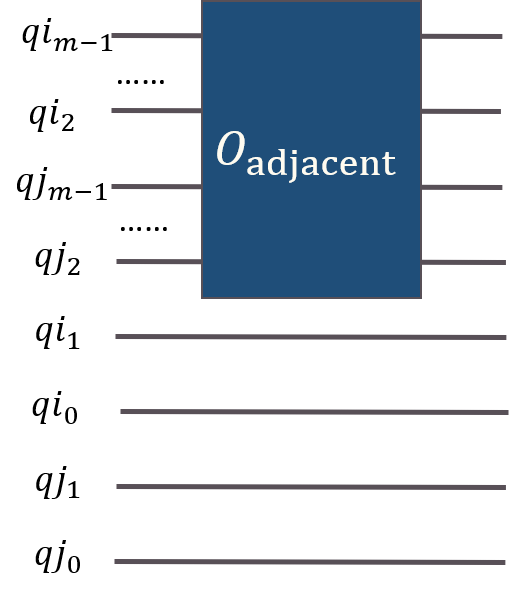
\includegraphics[width=0.30\textwidth]{Fig/OL.png}}
    \caption{$O_l$ quantum circuit. }
    \label{OL}
\end{figure}


\subsubsection{Oracle $O_b$}
$O_b$ can be written as:
$$
O_b|0\rangle=\sum_i{b_i|i\rangle}
$$
As shown in Sec.~\ref{classicalFVM}, the $\vec{b}$ represents the residual $\vec{R}$, and we find $R_i$ is a function of variables and coordinates of $(i/4)-th$ and its adjacent grids. In special, the expression of these functions is regular. In specific, $R_i$'s expression format is only related to $i\%4$, so we can efficiently construct $R_i$. To construct $O_b$, we need a QRAM which restores $\vec{U}$, we define:
$$
M_U|i\rangle|0\rangle=|i\rangle|U_i\rangle
$$

We can use $M_U$, $O_l$, $O_{coor}$ to construct $O_b$, as shown in fig.\ref{OB}, we first get the related variables and coordinates:
$$
|i\rangle|U_{related}\rangle|x_{related}\rangle
$$
Then, we compute $R_i$ and get
$$
|i\rangle|U_{related}\rangle|x_{related}\rangle|R_i\rangle
$$
Next, release $|U_{related}\rangle$ and $|x_{related}\rangle$,
$$
|i\rangle|R_i\rangle
$$
Finally, operate QDAC and we finish this process:
$$
\sum_i{b_i|i\rangle}
$$

\begin{figure}[htbp]
    \subfigure{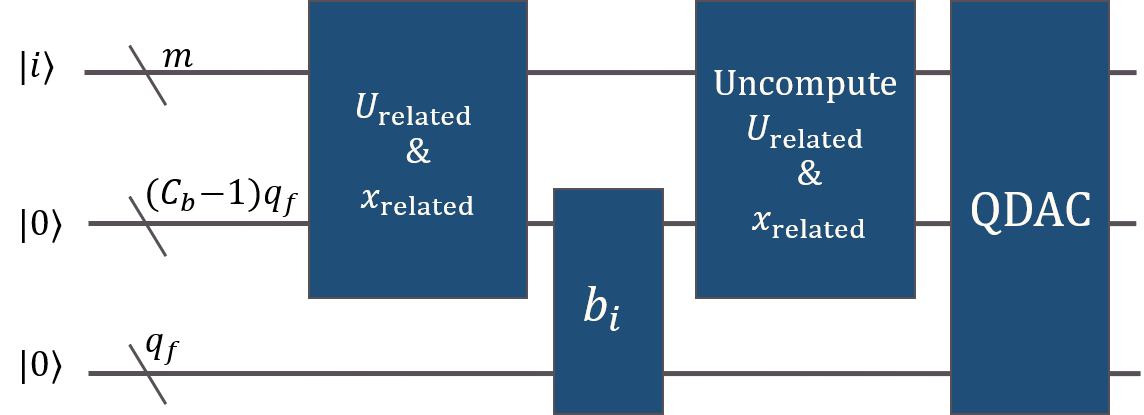
\includegraphics[width=0.30\textwidth]{Fig/Ob.png}}
    \caption{$O_b$ quantum circuit. }
    \label{OB}
\end{figure}

In this process, the required qubit number is $m+C_bq_f$, $C_bq_f$ is an ancilla qubit sequence used to compute $b_i$, it can also be used in QDAC quantum circuit. We assume the success rate of QDAC is $p_{QDAC}$, then the number of times $M_U$, $O_{adjacent}$ and $O_{coor}$ are used is $O(1/p_{QDAC})$. The gate complexity is $O(poly(m)/p_{QDAC}+poly(1/\epsilon p_{QDAC}))$, $\epsilon$ represents QDAC accuracy.


\subsubsection{Oracle $O_A$}
$O_A$ can be written as:
$$
O_A|i\rangle|j\rangle|z\rangle=|i\rangle|j\rangle|z\oplus A_{ij}\rangle
$$

To construct $O_A$, we also need $M_U$, $O_l$ and $O_{coor}$. As shown in Sec.\ref{classicalFVM}, matrix $A$ is a sparse matrix and the element $A_{4i_0+i_1,4j_0+j_1}\neq0$ only if grid $i_0$ and $j_0$ are adjacent, here $i_0,j_0\in[0,N-1]$ and $i_1,j_1\in[0,3]$, we have $i=4i_0+i_1$ and $j=4j_0+j_1$. $A_{4i_0+i_1,4j_0+j_1}$ is a function of variables and coordinates of grid $i_0$ and $j_0$, it can be written as
$$
A_{4i_0+i_1,4j_0+j_1}=f_{i_0,i_1,j_0,j_1}(\vec{u}_{i_0},\vec{u}_{j_0},\vec{x}_{i_0},\vec{x}_{j_0})
$$
Here the format of funcitons $f_{i_0,i_1,j_0,j_1}$ for different $i_0,i_1,j_0,j_1$ are also regular, it can be divided into two types:$i_0=j_0$ and $i_0\neq j_0$, and each type contains 16 conditions, corresponding to different $i_1$ and $j_1$. So we can efficiently construct $O_A$.

To compute $A_{4i_0+i_1,4j_0+j_1}$, we first construct
$$
|4i_0+i_1,4j_0+j_1\rangle|\vec{u}_{i_0},\vec{u}_{j_0},\vec{x}_{i_0},\vec{x}_{j_0}\rangle
$$
Then $f_{i_0,i_1,j_0,j_1}(\vec{u}_{i_0},\vec{u}_{j_0},\vec{x}_{i_0},\vec{x}_{j_0})$  is an arithmetic expression of $\vec{u}_{i_0},\vec{u}_{j_0},\vec{x}_{i_0},\vec{x}_{j_0}$, we get
$$
|4i_0+i_1,4j_0+j_1\rangle|\vec{u}_{i_0},\vec{u}_{j_0},\vec{x}_{i_0},\vec{x}_{j_0}\rangle|f_{i_0,i_1,j_0,j_1}(\vec{u}_{i_0},\vec{u}_{j_0},\vec{x}_{i_0},\vec{x}_{j_0})\rangle
$$
Finally, uncompute $\vec{u}_{i_0},\vec{u}_{j_0},\vec{x}_{i_0},\vec{x}_{j_0}$,
$$
|4i_0+i_1,4j_0+j_1\rangle|0,0,0,0\rangle|f_{i_0,i_1,j_0,j_1}(\vec{u}_{i_0},\vec{u}_{j_0},\vec{x}_{i_0},\vec{x}_{j_0})\rangle
$$
And we realize $O_A$, the corresponding quantum circuit is shown in fig.~\ref{OA} 
\begin{figure}[htbp]
    \subfigure{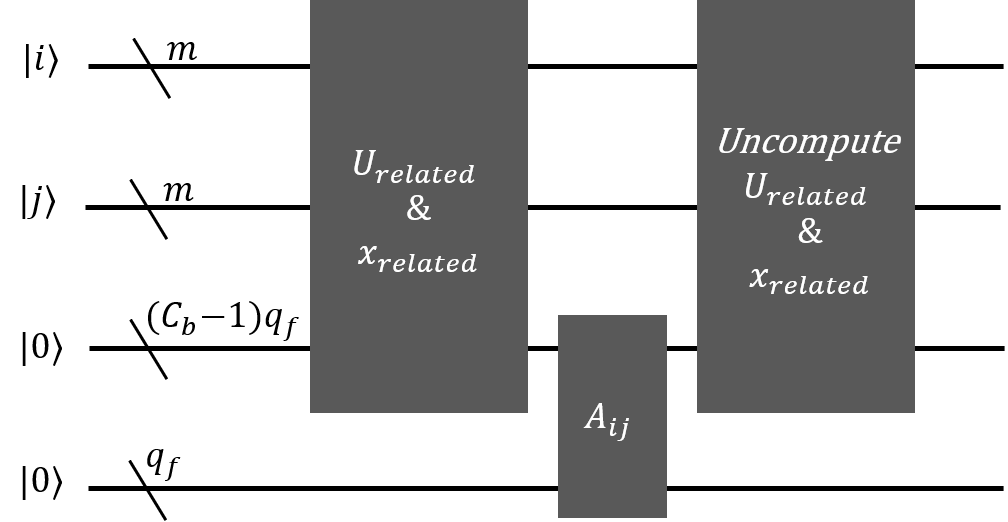
\includegraphics[width=0.30\textwidth]{Fig/OA.png}}
    \caption{$O_A$ quantum circuit. }
    \label{OA}
\end{figure}
In this process,the number of times $M_U$, $O_{adjacent}$ and $O_{coor}$ are used is $O(1)$. The required qubit number is $2m+C_Aq_f$, $C_Aq_f$ is a ancilla qubit sequence used to compute $A_{ij}$. The gate complexity is $O(poly(m))$. $A_{ij}$'s expression is more complicated than $b_i$, so $C_A>=C_b$, the qubit number used in $O_l,O_b,O_A$ is $2m+C_Aq_f$.

\subsection{necessity of QRAM}
\noindent Proposition I:Let $\left|\phi\right\rangle = \sum_{i=1}^n \left|u_i\right\rangle$ ($\left|u_i\right\rangle$ parallel to basis vectors and orthogonal each other). There exists 
linear transformation $A$ independent of $\left|u_{i}\right\rangle$ s.t. $\left|\psi\right\rangle = A\left|\phi\right\rangle$, iff $\left|\psi\right\rangle$ could express as $\sum_{i=1}^{n}\left|u_i\right\rangle\left|f\left(u_i\right)\right\rangle$.

\noindent Pf: 1.Necessity:Let $\left|\phi_i\right\rangle = \sum_{j=1}^n \left|x_{ij}\right\rangle$. If there exists linear transformation $A$ s.t.
\begin{align*}
A\left|\phi_i\right\rangle = \sum_{i=1}^n\left|x_{ij}\right\rangle\left|f_{j}\left(x_{i1}, x_{i2}, ..., x_{in}\right)\right\rangle
\end{align*}
then
\begin{align*}
A\sum_{i=1}^{n}\left|\phi_i\right\rangle = \sum_{i, j=1}^n\left|x_{ij}\right\rangle\left|f_{j}\left(x_{i1}, x_{i2}, ..., x_{in}\right)\right\rangle
\end{align*}
Rearrange the terms. We have: 
\begin{align*}
LHS = \sum_{i, j=1}^n\left|x_{ij}\right\rangle\left|f_{i}\left(x_{1j}, x_{2j}, ..., x_{nj}\right)\right\rangle = RHS
\end{align*}
Therefore,for all $\left(i, j\right) \in \left[1, n\right]\times\left[1, n\right]$, 
\begin{align*}
f_{j}\left(x_{i1}, x_{i2}, ..., x_{in}\right) = f_{i}\left(x_{1j}, x_{2j}, ..., x_{nj}\right)
\end{align*}
1)While $i=j$, $f_{i}\left(x_{i1}, x_{i2}, ..., x_{in}\right) = f_{i}\left(x_{1i}, x_{2i}, ..., x_{ni}\right)$, i.e., 
\begin{align*}
f_i\left(u_1, u_2, ...,u_n\right) = f_i\left(u_i\right)
\end{align*}
2)While $i\neq j$, $f_j\left(x_{ij}\right) = f_i\left(x_{ij}\right)$, i.e., 
\begin{align*}
f_i\left(u\right) = f\left(u\right)
\end{align*}
Above all, 
\begin{align*}
A\sum_{i=1}^{n}\left|u_i\right\rangle = \sum_{i=1}^{n}\left|u_i\right\rangle\left|f\left(u_i\right)\right\rangle
\end{align*}

2.Sufficiency: Obvious.

\noindent Proposition II:Let $\left|\phi\right\rangle = \sum_{i=1}^n \left|i\right\rangle\left|u_i\right\rangle$ ($\left|u_i\right\rangle$ parallel to basis vectors and orthogonal each other). There exists 
linear transformation $A$ independent of $\left|u_{i}\right\rangle$ s.t. $\left|\psi\right\rangle = A\left|\phi\right\rangle$, iff $\left|\psi\right\rangle$ could express as $\sum_{i=1}^n \left|i\right\rangle\left|u_i\right\rangle\left|f_{i}\left(u_i\right)\right\rangle$.

\noindent Pf: 1.Necessity:Let $S_n$ be the set of all cycle notations of permutation $\left(1, 2, ..., n\right)$. If there exists linear transformation $A$ s.t. 
\begin{align*}
	A\left|\phi\right\rangle = \sum_{i=1}^n \left|i\right\rangle\left|u_i\right\rangle\left|f_{i}\left(u_1, u_2, ..., u_n\right)\right\rangle
\end{align*}
then, for all $\left(j_1, j_2, ..., j_n\right)\in S_n$, 
\begin{align*}
	A\sum_{i=1}^n \left|i\right\rangle\left|u_{j_i}\right\rangle = \sum_{i=1}^n \left|i\right\rangle\left|u_{j_i}\right\rangle\left|f_{i}\left(u_{j_1}, u_{j_2}, ..., u_{j_n}\right)\right\rangle
\end{align*}
Therefore,  
\begin{align*}
	&A\sum_{\left(j_1, j_2, ..., j_n\right)\in S_n}\sum_{i=1}^n \left|i\right\rangle\left|u_{j_i}\right\rangle \\
	&=\sum_{\left(j_1, j_2, ..., j_n\right)\in S_n}\sum_{i=1}^n\left|i\right\rangle\left|u_{j_i}\right\rangle\left|f_{i}\left(u_{j_1}, u_{j_2}, ..., u_{j_n}\right)\right\rangle
\end{align*}
And
\begin{align*}
	LHS &= A\sum_{\left(j_1, j_2, ..., j_n\right)\in S_n}\sum_{i=1}^n \left|j_i\right\rangle\left|u_i\right\rangle\\
	&= A\sum_{i=1}^n\sum_{\left(j_1, j_2, ..., j_n\right)\in S_n}\left|j_i\right\rangle\left|u_i\right\rangle\\
	&= A\sum_{i=1}^n\sum_{k=1}^n\left|k\right\rangle\left|u_i\right\rangle \\
	&= \sum_{i=1}^n\sum_{k=1}^n\left|k\right\rangle\left|u_i\right\rangle\left|f_{k}\left(u_i, u_i, ..., u_i\right)\right\rangle\\
	&= \sum_{k=1}^n\sum_{i=1}^n\left|i\right\rangle\left|u_k\right\rangle\left|f_{i}\left(u_k, u_k, ..., u_k\right)\right\rangle \\
	&= \sum_{\left(j_1, j_2, ..., j_n\right)\in S_n}\sum_{i=1}^n\left|i\right\rangle\left|u_{j_i}\right\rangle\left|f_{i}\left(u_{j_i}, u_{j_i}, ..., u_{j_i}\right)\right\rangle\\
	&= RHS
\end{align*}
Corresponding items must be equal to each other, that is, for all $i \in \left[1, n\right]$ and $\left(j_1, j_2, ..., j_n\right)\in S_n$, 
\begin{align*}
	f_{i}\left(u_{j_1}, u_{j_2}, ..., u_{j_n}\right) = f_{i}\left(u_{j_i}, u_{j_i}, ..., u_{j_i}\right)
\end{align*}
i.e.,for any $i\neq j$
\begin{align*}
	\frac{\partial f_i\left(u_1, u_2, ..., u_n\right)}{\partial u_j} = 0
\end{align*}
in other, 
\begin{align*}
	f_i\left(u_1, u_2, ...,u_n\right) = f_i\left(u_i\right)
\end{align*}
Hence $A$ should meet the condition: 
\begin{align*}
	A\left|\phi\right\rangle = \sum_{i=1}^n \left|i\right\rangle\left|u_i\right\rangle\left|f_{i}\left(u_i\right)\right\rangle
\end{align*}

2.Sufficiency: Obvious.

\subsection{Quantum Linear Solver}

After the Linearization, we know change the problem into solving the linear
equation. Our goal is to output a state 
\begin{equation}
|\tilde{x}\rangle:=\frac{\Sigma_i \tilde{x}_i|i\rangle}
{\lVert \Sigma_i \tilde{x}_i |i\rangle\rVert}\notag
\end{equation}
such that, $\lVert |\tilde{x}\rangle-|x\rangle\rVert\leqslant\epsilon$. 
The amplitude of $|x\rangle$ satisfy $\vec{x}=A^{-1}\vec{b}$

\subsubsection{Overall Circuit and Qubit Number}
Base on the analyse above, the overall algorithm can be represented as 
following
\begin{figure}[htbp]
\centering
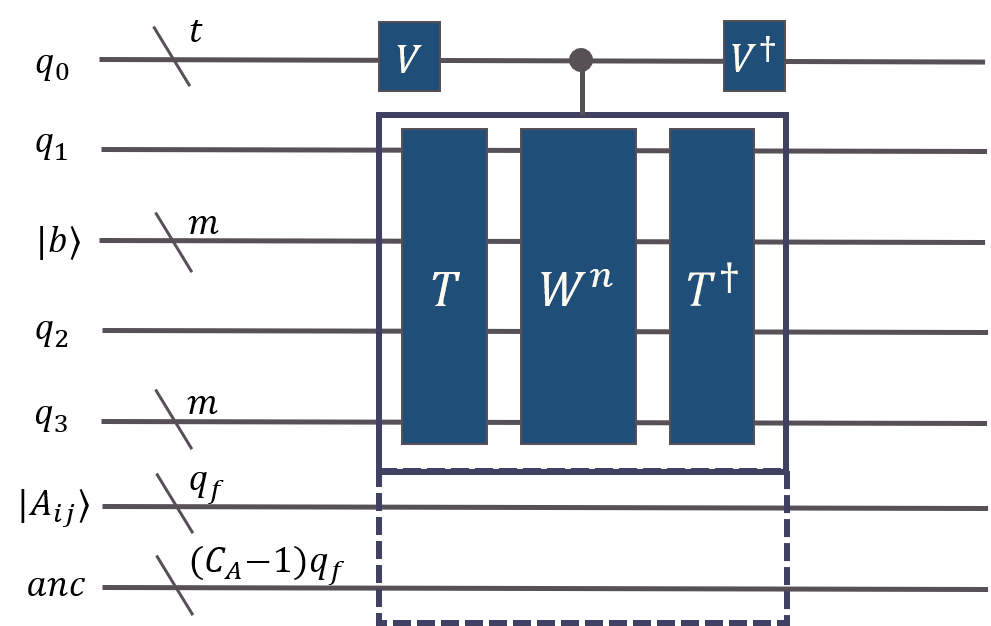
\includegraphics[width=0.4\textwidth]{Fig/overall}
\caption{The overall circuit}
\label{o}
\end{figure}

In fig.~\ref{o}, $t=O(log(j_0))$ is the qubits for control bits  $\frac{1}
{\sqrt{\alpha}}\sum_i\sqrt{\alpha_i}|i\rangle$. The total qubits number is $2(m+1)+t+C_Aq_f$

\subsubsection{Complexity and Successful probability}
In \cite{doi:10.1137/16M1087072}, function $1/x$ can be $\epsilon$ approximated by
linear combination of Chebyshev polynomials with highest order 
$O(j_0)=O(d\kappa log(d\kappa/\epsilon))$, the total
query complexity is $O(\alpha j_0)$. Because $\alpha\leqslant 4j_0/d$.
$O(\alpha j_0)=O(d\kappa^2log^2(d\kappa/\epsilon))$. The total number of 
$\mathcal{P}_B$ is $O(\alpha)$.

In \cite{7354428}, the gate complexity is $O(d\kappa^2log^2(d\kappa/
\epsilon)(logN+log^{2.5}(d\kappa/\epsilon))$
and the success probability is 
$(\lVert F|b\rangle\rVert/\alpha)^2$. 

Now the matrix F is the inverse of $A$ 
which has condition number $\kappa$ and $\lVert A\rVert=1$. 

So $\lVert F|b\rangle\rVert\in (1, \kappa)$. For $\alpha\leqslant4j_0/d$ so
$P_{succ}\geqslant 1/(16\kappa^2 log(d\kappa/\epsilon) log(4(\kappa d)^2log(d
\kappa/\epsilon)/\epsilon)$. 


\subsection{Postprocessing}

We got $\Delta \vec{U}^n$ through quantum linear solver. In postprocessing process, we update $M_U$. First, we operate QADC on $\Delta \vec{U}^n$ and get digital version of $\Delta \vec{U}^n$:
$$
d_{\Delta U}^n=\sum_i{|i\rangle|\Delta U_i^n\rangle}
$$
Then we construct the following state with $M_U$:
$$
\sum_i{|i\rangle|\Delta U_i^n\rangle|U_i^n\rangle}
$$
Next, execute adder on $|\Delta U_i^n\rangle$ and $|U_i^n\rangle$
$$
\sum_i{|i\rangle|\Delta U_i^{n+1}\rangle|U_i^n\rangle}
$$
Finally, release $|U_i^n\rangle$ with $M_U^{\dagger}$
$$
\sum_i{|i\rangle|\Delta U_i^{n+1}\rangle|0\rangle}
$$
The quantum circuit is shown as follows: FIG. \ref{postprocessing_qcir}
\begin{figure}[htbp]
	\subfigure{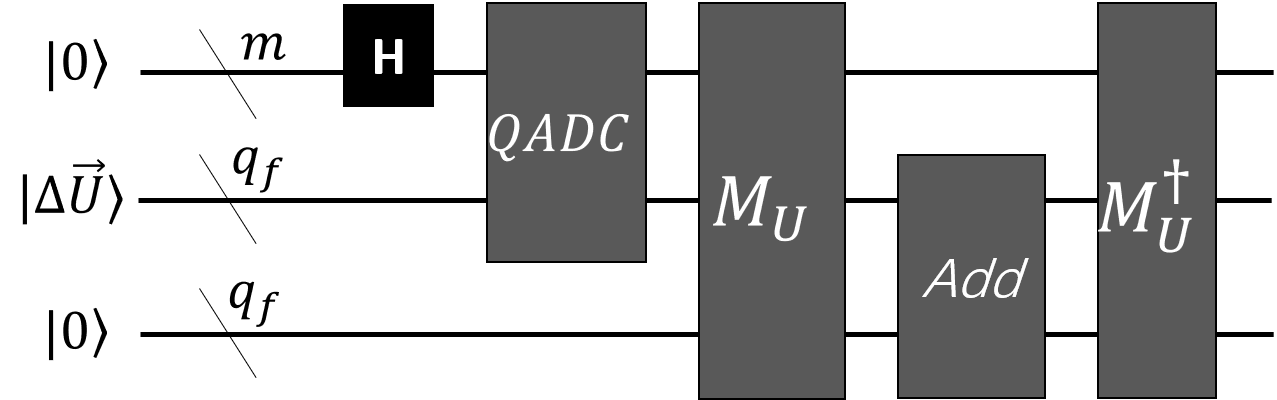
\includegraphics[width=0.48\textwidth]{Fig/postprocessing.png}}
	 \caption{The quantum circuit of the postprocessing.}
	\label{postprocessing_qcir}
   \end{figure}
We get the $d_U^{n+1}$ and update $M_U$ with $d_U^{n+1}$. In this process, the qubit number is $m+2q_f$. We use $M_U$ two times,QADC one time and execute quantum adder, the gate complexity is $O(poly(m))+L(QADC)$.


\subsection{classical information extraction}
Classical information extraction is the last step of our quantum algorithm. 
The final evolution of our algorithm is about digital-encoded states
$|\vec{U}\rangle$ which is stored in the QRAM. 
The process of classical information extraction is as follows: 
Read digital-encoded states $|\vec{U}\rangle$ from QRAM, 
then through QDAC becomes analog-coded state $\left| \psi  \right\rangle  = C\sum\limits_{k = 1}^N {{U_k}\left| k \right\rangle } $,
where $C = \sqrt {{1 \mathord{\left/
{\vphantom {1 {\left( {\sum\nolimits_{j = 1}^N {U_j^2} } \right)}}} \right.
\kern-\nulldelimiterspace} {\left( {\sum\nolimits_{j = 1}^N {U_j^2} } \right)}}} $.
Finally, measuring the analog-coded state $\left| \psi  \right\rangle $.

We use N grids during the calculation,
since the number of N is relatively large,
when sampling, we reduce the $N$ grids to $N_1$ grids, 
and then sample the $O(N_1)$ times to get the classical information of the final output.

Assume that the $j$-th grid after dimension reduction contains $a_j$ original grid,
a total of M times, the $j$-th grid appears $b_j$ times, then the output of the obtained $N_1$ grids can be expressed as: ${\vec u_{out}} = \left( {{{{b_j}} \mathord{\left/
{\vphantom {{{b_j}} {{a_j}}}} \right. \kern-\nulldelimiterspace} {{a_j}}}} \right),j = 0,1, \cdots ,{N_1} - 1$.

Finally we sample M times,
because QDAC is a probabilistic operation,
in other words, 
there is a probability that $p = \sum\nolimits_{j = 1}^N {{{U_j^2} \mathord{\left/
{\vphantom {{U_j^2} N}} \right. \kern-\nulldelimiterspace} N}} $ will successfully convert 
the digital-encoded information into analog-coded information,
thus we need $M/p$ times to extract information from QRAM and $M/p$ times QDAC.



\subsection{Overall Complexity Analysis}

In this section, we analyze the complexity of the entire algorithm flow. The required qubit number of the whole process is 
$$
qnum=2(m+1)+log(j_0)+C_Aq_f
$$
As shown before, $O(j_0)=O(d\kappa log(d\kappa/\epsilon))$.
In each iteration, two subprocesses might fail: QDAC operation in construction process of $O_b$ and linear combination of Chebyshev polynomials in construction process of $A^{-1}$. The success rates corresponding to these two subprocesses are written as:
$$
p_{QDAC}=\frac{1}{4N}\sum_i{(\Delta U_i/C_{max})^2}
$$

$$
p_{A^{-1}}=\frac{1}{\alpha}
$$
Here $C_{max}>=max\{\Delta U_i\}$ and $O(\alpha)=O(\kappa log(\kappa d/\epsilon))$. $p_{QDAC}$ is a constant number, we can ignore it.
Oracle $O_{adjacent}$ and $O_{coor}$ appear $O(1)$ times in quantum circuit of $O_l,O_b,O_A$, $O_l$,$O_A$ appear $O(j_0)$ times in each iteration. So the query complexity of $O_{adjacent}$ and $O_{coor}$ is $O(\alpha IterTimes\times j_0)$.

QRAM $M_U$ also appears $O(1)$ times to construct $O_b$ and $O_A$, the query complexity of $M_U$ is $O(\alpha IterTimes\times j_0)$. In each iteration, we update $M_U$, the update complexity of $M_U$ is $O(IterTimes)$.

The gate complexity of the whole process is $O(\alpha j_0poly(log(4N))/\epsilon)$.





\subsection{Normalization explanation}
As expected, linear systems like $\mathcal{A} \bm{\Delta U} = \bm{b}$ ($N$ variables) could be solved by quantum algorithms. But outputs are corresponding states instead of the actual root vectors. Different from vector $\bm{\Delta U}$, quantum state $\left| \Delta U\right\rangle$ has been normalized: 
\begin{align}
	\left| \Delta U\right\rangle = \frac{A^{-1} \left|b\right\rangle}{\left\|A^{-1} \left|b\right\rangle\right\|} = c A^{-1} \left|b\right\rangle = c \sum_{i=1}^{N} \Delta u_i\left|i\right\rangle
\end{align}

For different $A$ and $\left|b\right\rangle$, we have different normalization constants, i.e., $c^{n} \neq c^{n+1}$, usually. As described above, $U^{n+1}$ equals $U^{n} + \Delta U^{n} = U^{1} + \sum_{i=1}^{n} \Delta U^{i}$, which means performing operations like $\Delta U^{i} + \Delta U^{j}$ is necessary, yet there would be some trouble with accomplishing them by adding $\left|\Delta U^{i}\right\rangle$ to $\left|\Delta U^{j}\right\rangle$.

Consider there is a constant $L$ large enough, and construct a new state $\left|\Delta U^{\prime}\right\rangle$: 
\begin{align}
	\left|\Delta U^{\prime}\right\rangle = \sum_{i=1}^{N+1}\Delta  u_i^{\prime}\left|i\right\rangle
\end{align}
where
\begin{equation}
	\left\{
	\begin{array}{ll}
		\Delta u_i^{\prime} = \frac{\Delta u_i}{L}&,\ 1\leq i \leq N\\
		&\\
		\Delta u_i^{\prime} = \sqrt{1 - \sum_{j=1}^{N}{\Delta u_j^{\prime}}^2}&,\ i=N+1
	\end{array}
	\right.
\end{equation}

Then we got a new set of equations:
\begin{equation}\label{eq:Delta_u_prime_equations}
	\left\{
	\begin{array}{l}
		\sum_{j=1}^{N}A_{ij}\Delta u_j^{\prime} = \frac{b_i}{L} \ s.t. \ 1\leq i \leq N\\
		\\
		\sum_{i=1}^{N + 1}{\Delta u_i^{\prime}}^2 = 1
	\end{array}
	\right.
\end{equation}

To linearize Formula.\ref{eq:Delta_u_prime_equations}.2, we could replace ${\Delta u^{\prime n}_i}^2$ with $\Delta u^{\prime n - 1}_i \Delta u^{\prime n}_i$ while $\Delta t$ is small enough. And we gained new linear systems $\mathcal{A^{\prime}} \bm{\Delta U^{\prime}} = \bm{b^{\prime}}$: 
\begin{equation}
\begin{array}{cc}
	\mathcal{A^{\prime}} = \left[
	\begin{array}{cc}
		&\\
		\mathcal{A} & \bm{0}\\
		&\\
		\Delta u^{\prime n - 1}_1...\Delta u^{\prime n - 1}_N&\Delta u^{\prime n - 1}_{N+1}
	\end{array}
	\right]
	&
	\bm{b^{\prime}} = \left[
	\begin{array}{c}
		\frac{b_1}{L}\\
		...\\
		\frac{b_N}{L}\\
		1
	\end{array}
	\right]
	
\end{array}
\end{equation}
For state $\left|\Delta U^{\prime}\right\rangle$, the normalization constant is $1$ for ever. Then we could accomplish the math operations freely (using the first $N$ components of $\left|\Delta U^{\prime}\right\rangle$). While $N$ is large enough, $\mathcal{A^{\prime}}$ is also a sparse matrix. We could construct it efficiently.

\iffalse
Observing the Jacobi Matrix, we could found that except for boundaries, each variable appeared at least $3$ times in $\mathcal{A}$. Let $S_{var}$ be the set of orders of rows where variable $var$ appeared. As mentioned above, there are at most d nonzero entries in any row or column in $\mathcal{A}$, i.e., $\left\|S_{var}\right\|\leq d$. If there exists $var_i$ and $var_j\neq var_i$ such that $S_{var_j}\subset S_{var_i}$, we could use rows of which orders were in $S_{var_i}$ to eliminate the $i-th$ and $j-th$ entries of the last row of $\mathcal{A^{\prime}}$. 

If not, $var_i$ and $var_j$ are not independent in eqautions of which orders are in $S_{var_i}$,  which means $var_i$ and $var_j$ are not independent in the total linear systems, which couldn't be true. 

Because of $\left\|S_{var}\right\|\leq d$, we could construct a method to eliminate the entries of last row of $\mathcal{A^{\prime}}$: 1. $i=1$; 2. Using the corresponding $\left\|S_{var_i}\right\|$ to eliminate the $i-th$ entry; 3. $i=i+1$ until the $i-th$ entry hasn't been eliminated; 4. Back to step 2. 

Then we could eliminate at least $N/d$ entries of the last row of $\mathcal{A^{\prime}}$. Continue using equations without the $N/d$ variables to eliminate other entries. Finally, the number of nonzero entries in the last row would turn to $O(\sqrt{N})$, while $N$ is large enough.
\fi


\subsection{Relation to QRAM: The Main Difficulties of the Problem}

QRAM is a quantum analogue to the classical Random Access Memory (RAM). QRAM enables the user obtaining the data in the QRAM efficiently while the address is given in the superposition state. 
$$
QRAM: \sum_i{|i\rangle|0\rangle}=\sum_i{|i\rangle|U_i\rangle}
$$
The $U_i$ denotes the classical data encoded in the quantum states.

There were several QRAM models proposed in the previous works. A typical one is to implement the QRAM by a set of optical devices, requiring O(log N) operations (N denotes the memory length). Another more straightforward approach is to realize it with the decomposition of the quantum circuits. However, although the addressing part is realized in O(log N), the state generation part involves O(N) multi-controlled NOT gates, which should not be considered as an efficient plan.

We will introduce an efficiently QRAM only requiring O(log N) operations in our plan. We have to mention that the QRAM is never fabricated in real, which will be one of the drawbacks.

\subparagraph{Overall Complexity without QRAM} The classical problem has linear complexity, which greatly constrains the design of the quantum methods, especially quantum-classical hybrid methods. 

It is already known that, if someone wants to fully convert components in quantum states to a classical memory, it uses at least $O(n)$ times. The pure classical solver uses time integration, an iteration process being necessary. If the result is stored in the quantum states with any quantum solver, and we expect data transferred between each step of the iteration are classical, the “quantum-classical converter” process is inevitable and $O(n)$ time is consumed, and no acceleration exists (second case in the table.~\ref{tab2}).

For the fourth case of the table.~\ref{tab2}, we declare it impossible to implement such a plan in real. The problem is the complexity of the query of $O_A$ should be constructed from the previous solved vector $\vec{u}^{n-1}$. As we have mentioned above, $O_A$ is related to more than one component in $\vec{u}^{n-1}$ for each matrix element, and we will prove formally that this process cannot be implemented by a linear operator, which is considered as fundamental for the quantum mechanics. The proof is written in the Supplementary Information.

\section{Conclusion}

In this paper, we are answering the problem set 2: The Computational Fluid Dynamics. Our task is to replace some certain modules in the SU2 CFD Solver with quantum modules, forming a quantum-classical hybrid approach. The original classical solver uses Finite Volume Method, along with the iteration on time integration to obtain the result of the fluid equations. By multigrid method, the classical has the $O(n)$ complexity between each iteration steps, where n denotes the number of mesh grids. Therefore, quantum solver must have sublinear time complexity to observe the quantum speed-up.

We here use the quantum linear solver to accelerate the solution of the linear equations. In order to prepare all the data needed by the quantum linear solver, we choose to replace the core procedures in the CFluidIteration process. One is the MultiGrid\_Cycle, including the preprocessing and the equation solving, fully replaced by a quantum process. Another is the Preprocessing part, which links the data between two iteration steps, also replaced by a quantum process. Naturally, classical data is replaced by quantum data. The input mesh info should be made as a QRAM, which is frequently used in preprocessor. Most of the internal data during the calculation are no longer needed, because they are saved in quantum registers. The configuration data of the whole problem are considered as constants, which are used to generate the quantum program directly.

We finally obtain the time complexity of $O(\log N)$ with N the mesh number, exponential faster than the classical counterpart. The requirement of the qubit number, with ancillary qubit taken into consideration, is also $O(\log N)$ in our algorithm.

We declare our plan have three advantages. First, without changing the problem model, we realize exponential quantum speedup in this problem. Second, we fully discover the program of the SU2, properly finding the replacement that we have to do, implementing our algorithm with QPanda quantum programming framework and obtaining numerical results. These work infers that it is possible to realize our full plan in the future. Third, we do not ignore the quantum-classical data conversion interface problem, which we thought would be a blind point of many other plans, because What we are solve is a realistic problem. Our assumptions on the conversion between the quantum and the classical data are all have some base works. Besides, we made a proof on this problem, by showing the necessity of the QRAM and other assumputions, without which quantum speedup would never be achieved.

There are also drawbacks of our plan. First, the complexity of the quantum program, although growing with logarithm on the mesh number, is greatly exceeding any limit of the near-term quantum devices. That is, fault-tolerant quantum computing scheme must be realized to solve this problem. Second, our plan did not discuss the realizability of the QRAM, which we thought is not our task.

In conclusion, the computational fluid dynamics problem is possible to achieve speed-up with a fault tolerant quantum computer using our plan. We replace several modules in SU2 to adapt the quantum computer and classical computer, finally obtaining the complexity of both time and qubit resource with $O(\log N)$. We hope our work would be a guide to the future research of the application of quantum computing on the realistic problems.


% \section{Supplementary information}
% \subsection{quantum circuit modules}
% In this section, we introduce the quantum circuit modules used in our algorithm quantum circuit construction.


% \subsection{QDAC and QADC}
% Mitarai, Kitagawa, and Fujii \cite{mitarai_quantum_2019} gave a deterministic algorithm for quantum digital-to-analog conversion(QDAC) and quantum analog-to-digital conversion(QADC). We first introduce these two quantum circuit modules.
% \paragraph{QDAC}

% The purpose of QDAC is to change a quantum state encoded by numbers between $0$ and $1$ into the amplitude before the quantum state. So the QADC operation is defined by
% \[\frac{1}{{\sqrt N }}\sum\limits_{j = 1}^N {\left| j \right\rangle \left| {{d_j}} \right\rangle  \to C\sum\limits_{j = 1}^N {{d_j}{{\left| 0 \right\rangle }^{ \otimes m}}} }. \]

% The main idea of the QDAC algorithm is to turn the coefficients in front of each ground state through a rotation of auxiliary bits. Now we want to explain only the following three questions.

% Firstly, the probability of success. The QDAC algorithm has only a certain probability of success and a certain probability of failure in operation. If it fails, run the algorithm from scratch. After calculation, the probability of one-time success is $\sum\nolimits_{j = 1}^N {d_j^2/N} $\cite{mitarai_quantum_2019}.

% Secondly, we give the circuit diagram of the algorithm.

% \begin{figure}[htbp]
%  \subfigure{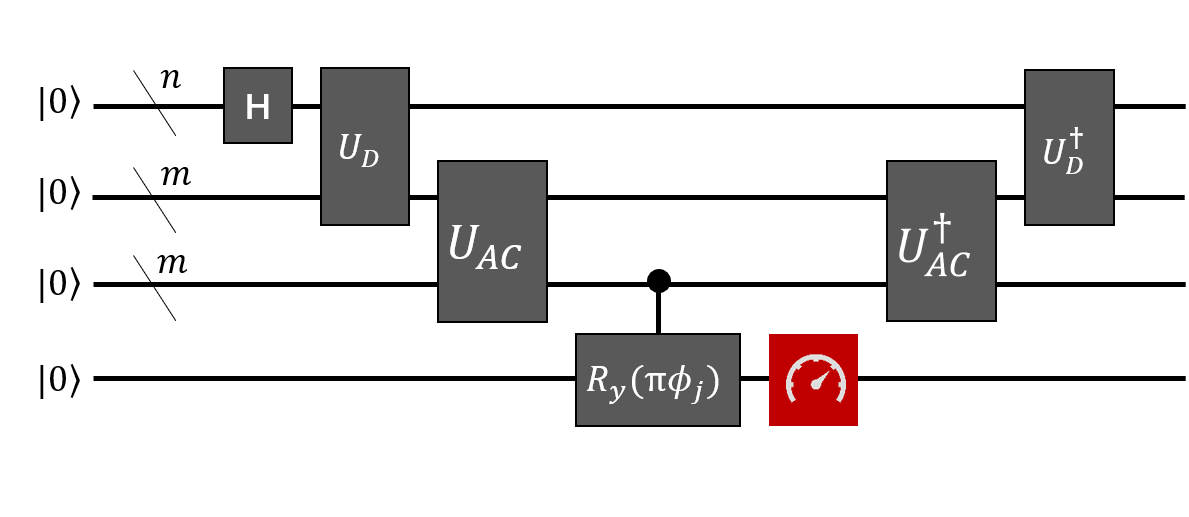
\includegraphics[width=0.48\textwidth]{Fig/qdac.png}}
%   \caption{The quantum circuit of the QDAC algorithms.(In measurement, if it is $\left| 0 \right\rangle $, continue; if it is $\left| 1 \right\rangle $, start from scratch.)}
%  \label{QDAC_qcir}
% \end{figure}

% The $n$ indicates the number of qubits required to encode data. The $m$ represents the number of digits of the desired precision. In the end, we only need to compute the upper bit. The function of ${U_D}$-gate is as follows:
% \[{U_D}\left( {\left\{ {{d_j}} \right\}} \right)\left| j \right\rangle \left| 0 \right\rangle  = \left| j \right\rangle \left| {{d_j}} \right\rangle \]

% The ${U_{AC}}$-gate means arccos function. The control-${R_y}$ gate represents the bit-by-bit control of rotation. If we don't consider $n$ H-gates, $O(m)$ gates are needed altogether \cite{mitarai_quantum_2019}.

% Thirdly, the normalization. Finally, the coefficients are needed to normalize. After calculation, the normalization coefficient $C$ is $\sqrt {1/\left( {\sum\nolimits_{j = 1}^N {d_j^2} } \right)} $ \cite{mitarai_quantum_2019}.


% \paragraph{QADC}

% Mitarai, Kitagawa, and Fujii \cite{mitarai_quantum_2019} gave a deterministic algorithm for a quantum analog-to-digital conversion(QADC).
% The algorithm includes absolute-QADC, real-QADC and imaginary-QADC.
% The main idea of these algorithms involves Hadamard test and phase estimation. The real-QADC is mainly used here. An $m$-bit real-QADC operation is defined by 
% $$
% {O_{rAD}}{\rm{:}}\sum\nolimits_{k = 1}^N {{c_k}\left| k \right\rangle {{\left| 0 \right\rangle }^{ \otimes m}}}  \to \frac{1}{{\sqrt N }}\sum\nolimits_{k = 1}^N {\left| k \right\rangle \left| {{{\tilde{\textbf x} }_k}} \right\rangle } ,
% $$
% where ${\tilde {\textbf x}_k}$ indicates the $m$-bit string $\tilde x_k^{\left( 1 \right)} \cdots \tilde x_k^{\left( m \right)}$ that best approximates the real part ${c_k}$ by $\sum\nolimits_{l = 1}^m {\tilde x_k^{\left( l \right)}{2^{ - l}}} $.

% The quantum circuit of the real-QADC algorithms is given as shown in FIG.\ref{QADC_fig}(a).

% \begin{figure}[htbp]
%  \subfigure[Real-QADC]{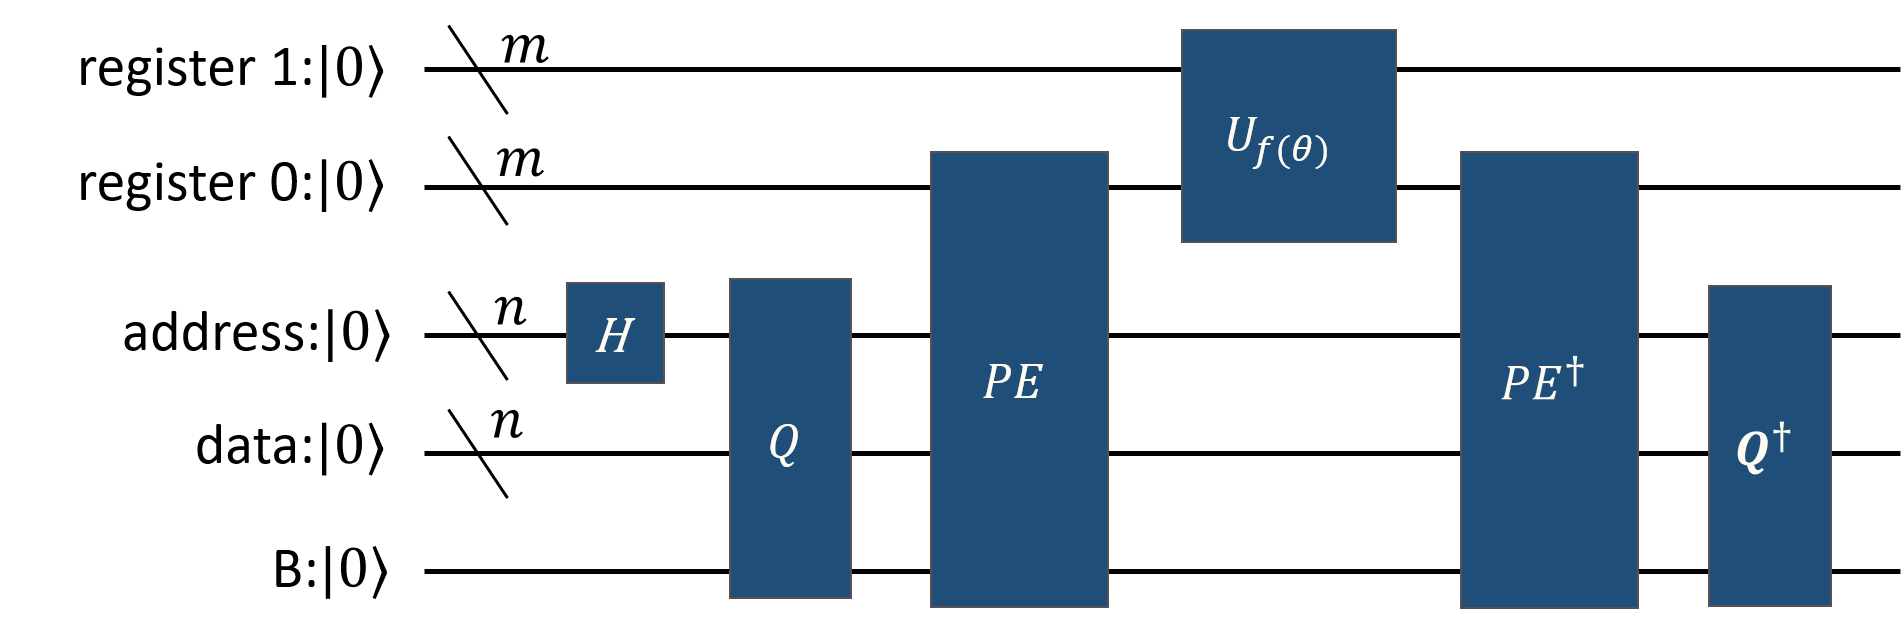
\includegraphics[width=0.50\textwidth]{Fig/real-QADC.png}}
%  \subfigure[Phase estimation]{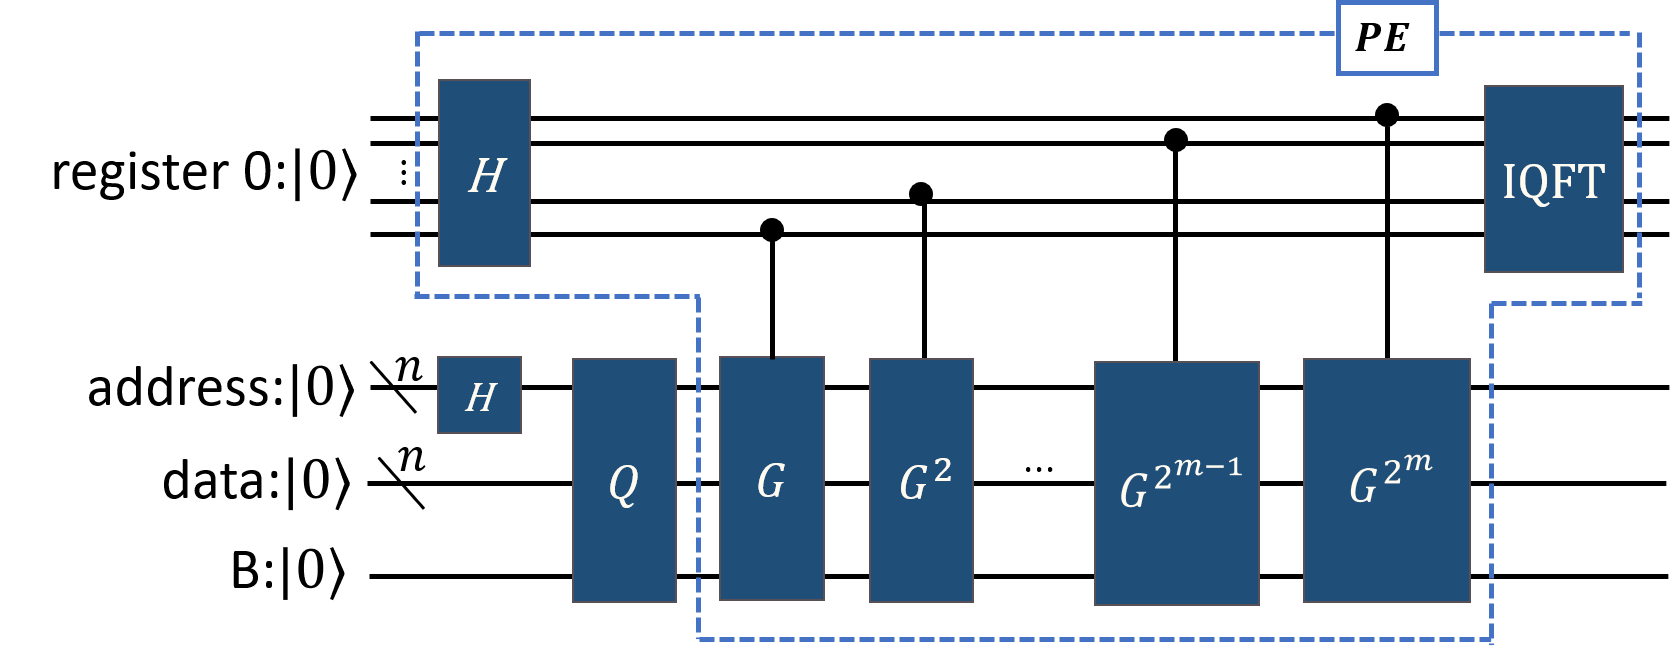
\includegraphics[width=0.45\textwidth]{Fig/PE.png}}
%  \subfigure[Quantum gate $W$]{\includegraphics[width=0.35\textwidth]{Fig/W.png}}
%  \caption{Quantum circuit: (a) the quantum circuit of the real-QADC algorithms, 
%  (b) the quantum circuit of phase estimation is in the blue dotted box
%  and (c) the part of quantum circuit of real-QADC, the green dotted box is $W$.}
%  \label{QADC_fig}
% \end{figure}

% $m$ and $n$ represent the number of digits of the desired precision and the number of qubits required to encode data, respectively.
% And an analog-encoding unitary transformation $U_A(\{c_j\})$ is defined by
% $${U_A}\left( {\left\{ {{c_j}} \right\}} \right)\left| 0 \right\rangle  = \sum\nolimits_j {{c_j}\left| j \right\rangle },$$
% where $\left\{ {{c_j}} \right\}_{j = 1}^N$ is classical data and normalized to satisfy $\sum\nolimits_{j = 1}^N {{{\left| {{c_j}} \right|}^2}}  = 1$.

% Gate G is given by
% $$G = W{S_0}{W^\dag }{Z_B},$$
% where $W$ is the gate shown in FIG.\ref{QADC_fig}(c), ${S_0} = I - 2{\left( {\left| 0 \right\rangle \left\langle 0 \right|} \right)_{data,B}}$
% is a conditional phase-shaft gate and ${Z_B}$ is a Pauli-$Z$ gate only acting on qubit $B$.

% PE indicates phase estimation ,IQFT means inverse quantum Fourier transformation\cite{nielsen_quantum_2002}.

% After phase estimation (PE), the phase ${\theta _k}$ of W can be encoded onto the register0 qubits, then use quantum arithmetics operation ${U_{f\left( \theta  \right)}}$ to calculate
% ${x_k} = f\left( {{\theta _k}} \right) = 2{\sin ^2}\pi {\theta _k} - 1$.
% Finally, the uncompute the data, B, reg0 qubits, the digital-coded state
% $\frac{1}{{\sqrt N }}\sum\limits_{k = 0}^N {{{\left| k \right\rangle }_{ad}}{{\left| {{{\tilde {\textbf x}}_k}} \right\rangle }_{reg1}}{{\left| 0 \right\rangle }_{reg0,data,B}}} $
% is obtained.


% From the quantum circuit of the real-QADC, $2(m+n)+1$ qubits are needed. Due to the gate $S_0$ can be split into $O[(log_{2}N)^2]$($N=2^n$) 
% single- and two-qubit gates\cite{barenco_elementary_1995}, thus the number of single- and two-qubit gates is $O[(log_{2}N)^2/{\epsilon}]$ and $O[1/{\epsilon}]$ $controlled-U_A$ gates are uesd\cite{mitarai_quantum_2019}.


% \subsubsection{Implementing the matrix inverse by linear combination of operators}
% Any simple function can be linear approximated by linear combination of other
% functions. We know want to approximate the inverse function of matrix by
% Chebyshev polynomials. In \cite{doi:10.1137/16M1087072} we know that 
% \begin{equation}
% \label{K}
% K|0^r\rangle|b\rangle=\frac{1}{\alpha}|0^r\rangle F|b\rangle
% +|\Xi^\bot \rangle\notag
% \end{equation}
% $K:=V^\dagger UV$, $U:=\Sigma_i|i\rangle\langle i|
% \otimes U_i$, 
% $V|0^m\rangle:=\frac{1}{\sqrt{\alpha}}\Sigma_i\sqrt{\alpha_i}|i\rangle$
% , $F=\Sigma_i\alpha_iG_i$
% , $\alpha:=\Sigma_i\alpha_i$, $r=m+t$ and 
% $(|0^r\rangle\langle0^r|\otimes\mathbbm{1})|\Xi_i^\bot\rangle=0$.

% In our problem, we need the inverse matrix function $f(x) = 1/x$, 
% it suffice that $O(\lVert A^{-1}-F\rVert)=\epsilon$.
% The linear combination\cite{doi:10.1137/16M1087072} is
% \begin{equation}
% g(x):=4\sum_{j=0}^{j_0}(-1)^j
% \frac{\sum_{i=j+1}^{b}\begin{pmatrix}
% 2b\\b+i
% \end{pmatrix}}{2^{2b}}\mathcal{T}_{2j+1}(x)\notag
% \end{equation}
% where $j_0=\sqrt{b log(4b/\epsilon)}$ and $b=\kappa^2log(\kappa/\epsilon)$.
% $g(x)$ is $2\epsilon$ close to $1/x$ on $D_\kappa:=(-1,-1/\kappa)\cup
% (1/\kappa,1)$.
% $\mathcal{T}_{2j+1}(x)$ is the Chebyshev polynomials of the first kind.
% \paragraph{Quantum Walk}
% To implement the Chebyshev polynomials, we should do it in a quantum walk 
% framework. 

% Because the quantum walk performed using a set of states $|\psi_j\rangle$
% in space $\mathbbm{C}^{2N}\otimes
% \mathbbm{C}^{2N}$.
% We have to define a map $T:=\sum_{j\in [N]}|\psi_j\rangle\langle j|$ from
% $\mathbbm{C}^{N}$ to $\mathbbm{C}^{2N}\otimes\mathbbm{C}^{2N}$.
% \begin{equation}
% |\psi_j\rangle:=|j\rangle\otimes \frac{1}{\sqrt{d}}
% \sum_{k\in [N]:A_{jk}\neq 0}(\sqrt{A^*_{jk}}|k\rangle+\sqrt{1-|A_{jk}|}|k+N
% \rangle)\notag
% \end{equation}
% and the walk operator
% \begin{equation}
% W=S(2TT^\dagger-1)\notag
% \end{equation}
% The operator $S$ perform the swap operation of the product states in 
% $|\psi_j\rangle$. Then we can get 

% \begin{equation}
% T^{\dagger}W^nT|b\rangle=|0^m\rangle\mathcal{T}_n(H)|b\rangle+|\bot_b\rangle\notag
% \end{equation}
% $\mathcal{T}_n(\lambda)$ is the first kind of Chebyshev polynomials.

% \paragraph{Quantum Circuit Implement}
% We use two oracles to extract information of matrix $A$: $O_l$ and $O_A$, which are written as:
% \begin{align}
% &O_l|j,l\rangle=|j,f(j,l)\rangle\notag\\
% &O_A|j,k,z\rangle=|j,k,z\oplus A_{jk}\rangle\notag
% \end{align}


% Our first goal is to encode the state $\frac{1}
% {\sqrt{\alpha}}\sum_i^{j_0}\sqrt{\alpha_i}|i\rangle$, it can be prepared with a $O(j_0)$-length quantum circuit.

% Then we construct operator $T$, as shown in \cite{7354428}, the operator $T$ can be synthesised as following.
% The whole circuit need $log_2(2N)$ qubits for vector $|j\rangle$, likewise 
% $log_2(2N)$ for its product states and a bunch of auxiliary qubits serve as 
% control rotation.

% \begin{itemize}
% \item $|0^t\rangle\xrightarrow{H}
% \frac{1}{\sqrt{d}}\sum_{l=0}^{d-1}|l\rangle$
% \item $|j\rangle\frac{1}{\sqrt{d}}\sum_{l=0}^{d-1}|l
% \rangle\xrightarrow{O_F}|j\rangle\frac{1}{\sqrt{d}}\sum_{l\in F_j}|l
% \rangle$
% \item $|j\rangle\frac{1}{\sqrt{d}}\sum_{l\in F_j}|l\rangle|0\rangle
% \xrightarrow{O_H}|j\rangle\frac{1}{\sqrt{d}}\sum_{l\in F_j}|l\rangle
% |A_{jl}\rangle$
% \item consider the $A_{jl}$ as a sequence of control bit, define a control 
% rotation operator

% \begin{equation}
% M:=\begin{pmatrix}
% \sqrt{H_{jl}^*/X} & -\sqrt{(1-|H_{jl}|)/X}\\
% \sqrt{(1-|H_{jl}|)/X} &\sqrt{H_{jl}^*/X}\notag
% \end{pmatrix}
% \end{equation}
% $|H_{jl}\rangle|0\rangle\xrightarrow{M}|H_{jl}\rangle
% \sqrt{H_{jl}^*/X}|0\rangle+\sqrt{(1-|H_{jl}|)/X}|1\rangle\notag$

% In \cite{PhysRevLett.122.020502}, operator $M$ can be synthesised by an oracle $O_{amp}$
% \begin{equation}
% |l\rangle|z\rangle\xrightarrow{O_{amp}}|l\rangle|z\otimes\alpha_l^{(n)}
% \rangle\notag
% \end{equation}
% Our goal is to prepare an approximation to the target state
% \begin{equation}
% |target\rangle:=\frac{1}{{\lVert\vec{\alpha}\rVert}_2}\sum_{l=0}^n\alpha_l
% |l\rangle\notag
% \end{equation}
% The key contributor is a operator $M$ as a control rotation operator.
% \begin{equation}
% |\alpha\rangle|0\rangle:=|\alpha\rangle(sin(\theta)|0\rangle+
% cos(\theta)|1\rangle)\notag
% \end{equation}

% \item apply the $O_H$ again to change the $|H_{jl}\rangle$ back to 
% $|0\rangle$.
% \end{itemize}

% \begin{figure}[h]
% \centering
% 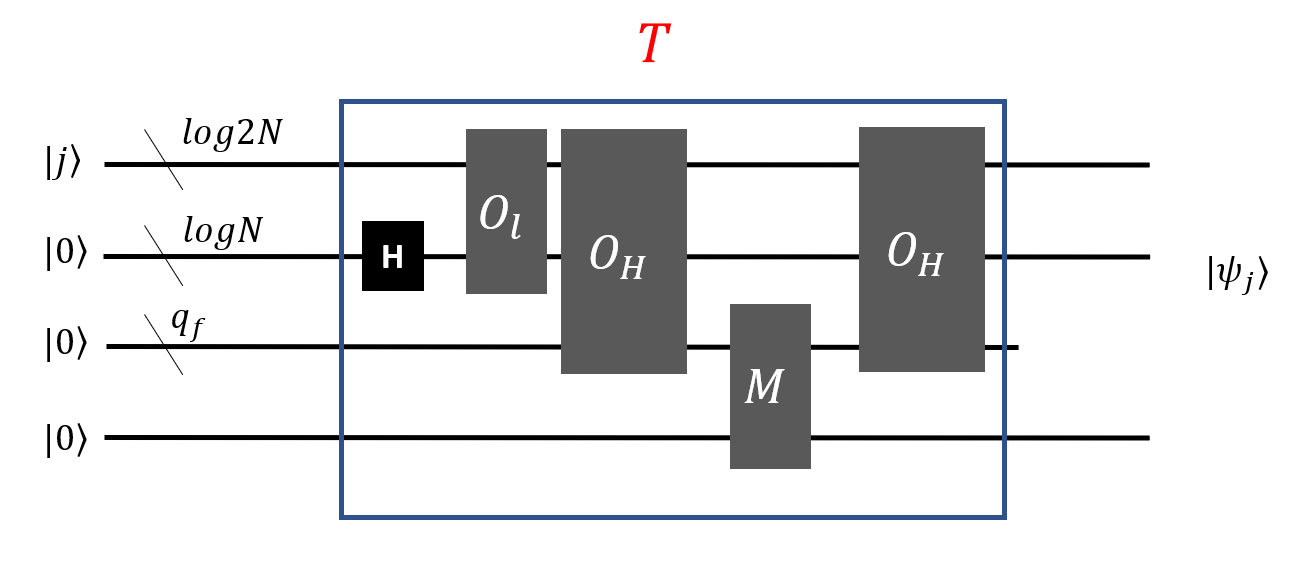
\includegraphics[width=0.45\textwidth]{Fig/T}
% \caption{Quantum circuit of Operator T}
% \label{T}
% \end{figure}

% Next, we show the quanutum circuit of operator $W$. Since $W=S(2TT^\dagger-I_{4N^2})$, $S$ can be easily constructed by a bunch of swap operators.
% What left to be done is $2TT^\dagger-I_{4N^2}$. 
% \begin{align}
% |\psi_j\rangle&=|j\rangle\otimes\frac{1}{\sqrt{d}} 
% \sum_{k\in [N]:A_{jk}\neq 0}(\sqrt{A^*_{jk}}|k\rangle+\sqrt{1-|A_{jk}|}|k+N
% \rangle)\notag\\
% &=|j\rangle\otimes|\phi_j\rangle\notag
% \end{align}
% so $TT^\dagger=|j\rangle\langle j|\otimes|\phi_j\rangle\langle\phi_j|$.
% The operator $T$ is a unitary in the quantum circuit which change
% the state $|j\rangle|0\rangle$ to $|\psi_j\rangle$. It is different from the
% $T:=\sum_{j\in[N]}|\psi_j\rangle\langle j|$ with dimension $4N^2\times2N$.
% To distinguish, we denote the quantum circuit by $T_{qc}$.
% \begin{align}
% &T_{qc}(\sum_j|j\rangle\langle j|\otimes(2|0\rangle\langle0|-I_{2N}))
% T_{qc}^\dagger=\notag\\
% &\sum_j|j\rangle\langle j|\otimes
% (2|\phi_j\rangle\langle \phi_j|-I_{2N})=2TT^\dagger-I_{4N^2}\notag
% \end{align}
% \begin{align}
% N&=2|0\rangle\langle0|-I_{2N}\notag \\
% &=diag(1,-1,-1,\dots,-1)=-diag(-1,1,1,\dots,1)\notag
% \end{align}
% \begin{figure}[htbp]
% \centering
% 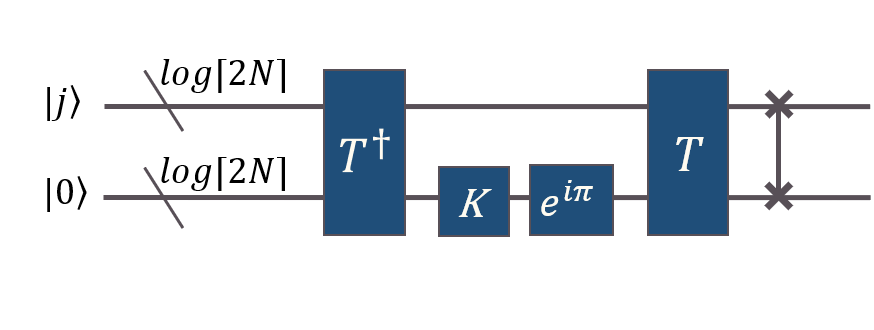
\includegraphics[width=0.4\textwidth]{Fig/WW}
% \caption{The operator $W$}
% \label{W}
% \end{figure}




\bibliography{cfd_aps}
\end{document}
